\clearpage
\section{Kinematical modelling}
\label{sec:kinematical_modelling}

\subsection{Velocities maps}

The velocity field and dispersion maps we used for our modelling, as well as flux and $\rm{SNR}$ maps, were produced with CAMEL\footnote{https://bitbucket.org/bepinat/camel.git} code. Sub-cubes extracted around the galaxies were first smoothed with a 2D spatial Gaussian (smoothing $\rm{FWHM}$ below the PSF $\rm{FWHM}$ to not drastically reduce the spatial resolution) in order to increase the $\rm{SNR}$ per pixel. A Gaussian profile, and a constant continuum, was then fitted onto every pixel around the [OII] lines. The 3D variance maps produced during the MUSE data reduction were used to weight the contribution of noise induced by sky line residuals. Velocity fields were computed as the average value of the Gaussian in every pixel, and the dispersion maps as the Gaussian dispersion (in velocity space).

\subsection{Manual cleaning}
\label{sec:manual_cleaning}

For every selected galaxy, we ran the automatic cleaning routine as described in Section \ref{sec:selecting_galaxies}. Cleaned maps were produced and the velocity maps were visually inspected. Isolated pixels were removed, even the very few with an identifiable [OII] doublet. We also inspected these lines near the edges and we removed any pixel whose velocity seemed inconsistent with that of its neighbours (typically a velocity offset around $50 - \SI{100}{\kilo\meter \, \second^{-1}}$). Twelve galaxies were found to be spatially unresolved with MUSE despite being selected, and $3$ were too close to the edges of the MUSE fields which resulted in missing data. Relaxing the $\rm{SNR}$ threshold in the routine to $3$ allowed us to recover $6$ galaxies out of $12$.



\subsection{Velocity field model}
\label{subsec:model}
\subsubsection{Ramp model}
\label{subsec:ramp_model}

In order to derive the kinematical parameters of our galaxies, we must fit a 2D velocity model onto the cleaned velocity fields. Galaxies kinematical models tend to describe the movement of gas by assuming circular rotation in the plane of the galaxy. The inclination of the galaxy on the sky will have the effect to bend the velocity field and produce a 'spider-diagram' (see Appendix \,\ref{sec:vel_decompo} for more details and Fig.\,\ref{fig:velocity_map} for an example). A few different models exist which might yield slightly different results. Some are derived assuming a certain mass distribution such as \shortciteA{Freeman1970} model of a thin exponential disc. Others rely on a visual description of observed galaxy rotation curves such as the 'ARCTAN' function of \shortciteA{Courteau1997} or the linear ramp model from \shortciteA{Wright2009} and \shortciteA{Epinat2012}.\\


We chose the linear ramp model to describe our velocity fields as it was found to better describe simulated galaxy rotation curves at high redshift

\begin{equation}
	V(R) = V_{\rm{s}} + V_{\rm{c}}  \times
	\begin{cases}
 		R / R_{\rm{c}} &\mbox{if } R < R_{\rm{c}} \\
		1 &\mbox{if }  R \geq R_{\rm{c}}
	\end{cases}
\end{equation}

This simple model consists in a linearly increasing slope in the central part till it reaches a radius $R_{\rm{c}}$ (turnover radius) beyond which the rotation velocity $V_{\rm{c}}$ remains the same (plateau). Such a modelling will only work under the assumption of the existence of a measurable global rotation. We also do not take into account features such as a central bar, spiral arms or clumps which are resolved for some galaxies in HST-ACS images. This is because of the lack of spatial resolution in our MUSE data which prevents us from clearly distinguishing these components in the kinematics. \\

We have in total $3$ fixed input parameters which must be known in advance: the inclination, and the centre right ascension and declination. The inclination is used by the model to appropriately bend the velocity field. As discussed in Appendix \ref{sec:vel_decompo}, there is a degeneracy between the maximum rotation velocity and the inclination of the galaxy so that the kinematical model would not converge to reliable values of $i$ if it were to freely vary. The free parameters are the systematic velocity $V_{\rm{s}}$, the turnover radius and the plateau velocity. 


%\newpage
\subsection{Beam-smearing and sampling effect on the dispersion}
\label{sec:beam_smearing_effect}

\subsubsection{The impact of beam-smearing}

The measured velocity dispersion in each pixel is affected both by the real dispersion related to local turbulent motion on the line of sight and by instrumental effects called beam-smearing. If we want to perform statistics on our morpho-kinematics parameters, such as computing a distribution for $V_{\rm{max}} / \sigma_{\rm{v}}$ which we can then use to study the Tully-Fisher Relation (TFR) of our sample, we need to derive a physically meaningful value of the average or median velocity dispersion. Our model takes into account this effect when computing a dispersion, but also for the velocity field which will also be impacted by beam-smearing effects. We give, in what follows, a description of the correction applied for the dispersion. This can be easily extended for velocity moments of any order. For more detailed information on the model, we refer to \shortciteA{Epinat2010} from which it is based.

\subsubsection{Formalism for the velocity field and dispersion maps}
\label{sec:vel_field_and_disp_map}
The velocity field is defined as the first moment of the emitting line ([OII] doublet in our case)

\begin{equation}
	V(x,y) = \int_\lambda L(x,y,\lambda) v(\lambda) d\lambda / M(x, y)
	\label{eq:vel_field_def}
\end{equation}
where $L(x, y, \lambda)$ is the line spectral light distribution and $M(x,y) = \int_\lambda L d\lambda$ the line flux (zero order moment). On the other hand, the velocity dispersion map is defined as the square root of the (central) second order moment

\begin{equation}
	\sigma_{\rm{v}} (x,y) = \left ( \overline{V^2(x,y)} - \overline{V(x,y)}^2 \right )^{1/2}
	\label{eq:disp_field_def}
\end{equation}
where $\overline{V^2(x,y)}$ is defined as in Eq.\,\ref{eq:vel_field_def} with $v \rightarrow v^2$. However, we have in practice a spectrum with a finite resolution due to spectral sampling. Thus, if we have $N$ contiguous spectral channels $\lbrace \lambda_i \rbrace_{i\leq N}$, and if the line is spectrally resolved, we can rewrite Eq.\,\ref{eq:vel_field_def} and \ref{eq:disp_field_def} with a discrete summation instead of an integral

\begin{equation}
	\overline{V(x,y)} \approx \sum_{i \leq N} S_i(x,y,\lambda_i) v(\lambda_i) / M(x, y)
	\label{eq:vel_field_def_sampled}
\end{equation}
where $S_i(x,y,\lambda_i)$ will be the spectral light distribution in the spectral channel centred on $\lambda_i$ and $M(x,y) \approx \sum_i S_i$.


%\newpage
\subsubsection{Impact of the PSF and LSF}
\label{sec:impact_PSF}

The light distribution in each channel will be convolved first by the LSF and then with the PSF so that $S_i^{\rm{0}} = S_i * \rm{LSF} * \rm{PSF}$ and $M_{\rm{0}} = M * \rm{LSF} * \rm{PSF}$. Any raw velocity moment of order $\alpha$ can be computed by substituting $S_i \rightarrow S_i^{\rm{0}}$ and $M \rightarrow M_{\rm{0}}$ in Eq.\,\ref{eq:vel_field_def} with $v \rightarrow v^{\alpha}$

\begin{equation}
	\overline{V_0^{\alpha}} = \left [ \left ( \overline{V^{\alpha}} M \right ) * \rm{PSF} \right ] / M_0
	\label{eq:raw_moment}
\end{equation}

Given Eq.\,\ref{eq:raw_moment}, we can compute the effect of the spatial PSF on the velocity dispersion

\begin{equation}
	\begin{split}
		\sigma_0^2 & = \overline{V_0^2} - \overline{V_0}^2 \\
		& = \left [ \frac{\left ( \sigma^2 + \overline{V}^2 \right ) M}{M_0} \right ] * \rm{PSF} - \left [ \left (  \frac{\overline{V} M}{ M_0} \right ) * \rm{PSF} \right ]^2
	\end{split}
\end{equation}

\subsubsection{Spatial sampling}
\label{sec:spatial_sampling}

The second effect to take into account is spatial sampling. The spectral light distribution is now spatially discretized as follows

\begin{equation}
	\begin{split}
		S_1 ( x_j , y_k , \lambda_i ) & = (\Delta x \Delta y)^{-1}\int_{\rm{pixel}} S_i^0 (x, y, \lambda_i) dx dy \\
		& = \left \langle S_i^0 (x, y, \lambda_i) \right \rangle_{(x_j , y_k)}
		\label{eq:spatial_sampling_on_light}
	\end{split}
\end{equation}
so that it corresponds to the average integrated light in a pixel centred on $(x_j , y_k)$ of width $\Delta x$ and height $\Delta y$. By summing Eq.\,\ref{eq:spatial_sampling_on_light} over all pixels, one recovers the total flux as

\begin{equation}
	M_1 (x_j , y_k ) = \left \langle M (x,y) * {\rm{PSF}} \right \rangle_{(x_j , y_k)}
\end{equation}
and more generally any raw velocity moment of order $\alpha$ will be written as

\begin{equation}
	\overline{V_1^{\alpha}} ( x_j , y_k) = \left \langle \left [ \frac{M \overline{V^{\alpha}}}{M_1} \right ] * {\rm{PSF}} \right \rangle_{(x_j , y_k)}
\end{equation}

This finally gives us the expression for the measured velocity dispersion affected by beam smearing effects and spatial sampling

\begin{equation}
	\sigma_{\rm{v}}^{\rm{obs}} (x_j , y_k ) = \left [ \left \langle \left [ \frac{\left (\sigma_{\rm{v}}^2 + \overline{V}^2 \right ) M}{M_1} \right ] * \rm{PSF} \right \rangle_{(x_j , y_k)} - \left \langle \frac{\overline{V}M}{M_1} * \rm{PSF} \right \rangle_{(x_j , y_k)}^2 \right ]^{1/2}
	\label{eq:sigma_obs}
\end{equation}

We see in Eq.\,\ref{eq:sigma_obs} that we need to know the best-fit velocity field model of our galaxy, as well as the PSF, to invert it and retrieve the real velocity dispersion map $\sigma_{\rm{v}}(x,y)$ from the observed one. The main limitation is that we need to know the flux distribution with high resolution, which we do not necessarily have in practice.



\subsection{Modelling}

\begin{figure}[htbp]
	\centering
	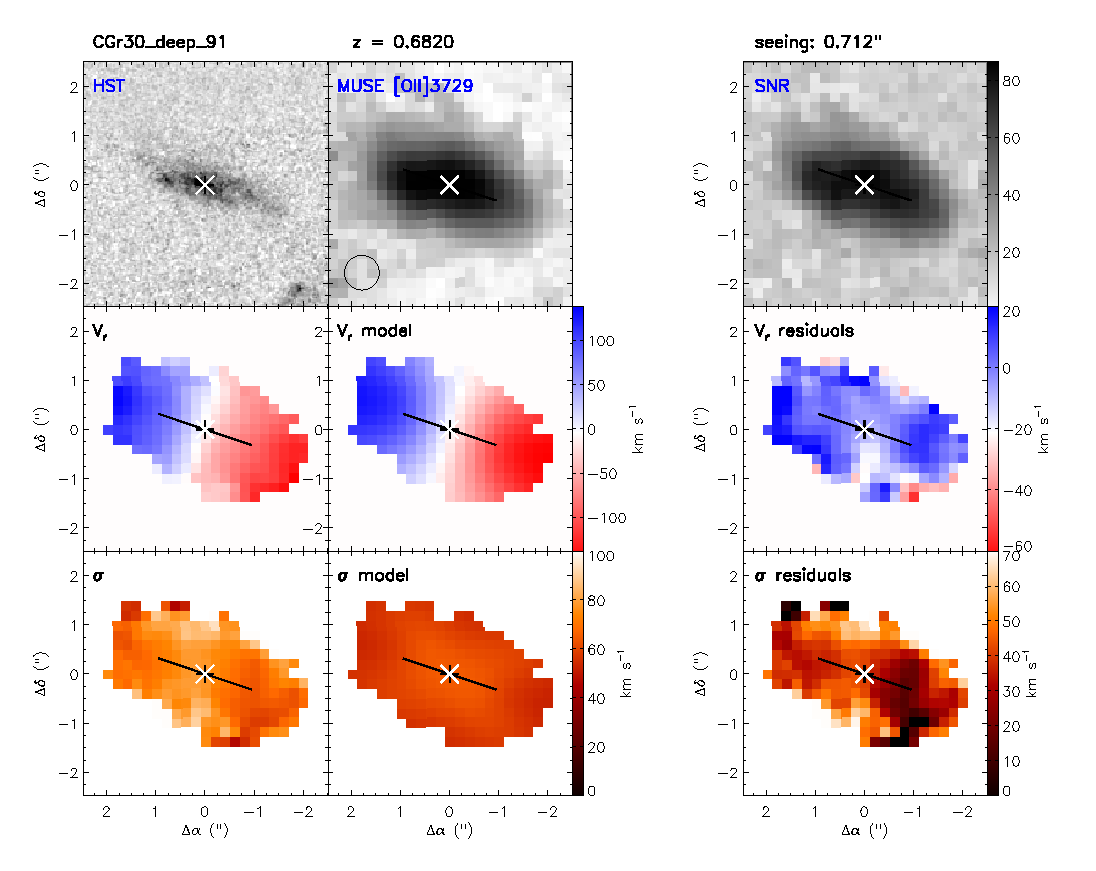
\includegraphics[width=0.85\linewidth]{{Figures/maps_CGr30_deep_91_o2_paper}.eps}
	\caption[Example of a kinematical model]{An example of the kinematical model for the galaxy \texttt{Gr30\_deep\_91}. North is up and East is left. The redshift of the galaxy and the PSF $\rm{FWHM}$ (seeing) at the observed wavelength are given on top. A circle of radius equal to the $\rm{FWHM}$ is also represented on top of the MUSE image. From left to right we show
		\begin{enumerate*}[label=]
			\item Top: HST-ACS image, MUSE [OII] narrow-band image and associated SNR map.
			\item Middle: observed [OII] velocity field from MUSE, velocity model and residuals between the two.
			\item Bottom: [OII] dispersion map from MUSE, dispersion model of the beam-smearing effect and the residual map corrected of the LSF.
		\end{enumerate*}		
	  The maximum rotational velocity is deduced from the kinematical parameters of the velocity field model. The velocity dispersion is computed from the residual map of the dispersion.}
	\label{fig:velocity_map}
\end{figure}

We applied the kinematical model and the beam-smearing correction described in previous sections on the $\sim 100$ field galaxies of our sample with an IDL routine, from B. Epinat, based on the Markwardt MPFIT IDL library. This code uses a reduced $\chi^2$ method with the Levenberg-Marquardt algorithm to fit a ramp model on the velocity field, and computes from it the dispersion map after accounting for beam-smearing effects. The derived morphological and kinematical parameters are given in Tables \ref{table:params1}, \ref{table:params2} and \ref{table:params3}. \\

We inspected the model against the velocity field for every galaxy, especially the centre position. We expected a couple of MUSE fields to have centre position offsets because of astrometry issues during the data processing. Thus, whenever the centre did seem offset, we moved it in a $3\times \SI{3}{px}$ box and searched for the position with the best $\chi^2$. The model converged in all cases except for the galaxy \texttt{CGr\_61\_134}. By lack of time, we did not investigate it further and we removed it from the analysis. Our model fits quite well the velocity fields for most of our sample except for $6$ galaxies with high $\chi^2$ values, which is due to their disturbed kinematics. An example of a kinematical model is given in Fig.\,\ref{fig:velocity_map} for \texttt{Gr30\_deep\_91}. This is a quite extended galaxy compared to others, at intermediate redshift and with a smooth velocity field. We also flagged $10$ galaxies which had poor spatial resolution compared to the remaining sample (generally because of low $\rm{SNR}$).